%   Filename    : chapter_4.tex 
\chapter{Preliminary Results/System Prototype}

\section{Model Evaluation}
\subsection{Model Training}
The model was trained for 7 epochs before the early stopping callback was triggered because the evaluation metrics has not improved by at least 0.01 for 3 consecutive epochs. This prevented the overfitting seen in the following figure. 
% {Insert Figure here}

Here, we can see that the while the training loss is decreasing, the validation loss is increasing and other metrics are not improving. This indicates that the model is overfitting to the training data and may not generalize well to new data. The model training was stopped in just 7 epochs and the best model amongst the epochs, the one with the lowest validation loss and highest metrics, was chosen as the final model.

\subsection{Text Generation}
A total of 197 sentences were translated using both the base zephyr-7b-beta model and the finetuned model. These served as the dataset used to evaluate the performance of the model and comparing it with the other base model.
\subsection{Automatic Evaluation Metrics}
The dataset was automatically evaluated using BLEU and ROUGE metrics, specifically the ROUGE-L metric as the dataset do not contain newlines that ROUGE-Lsum uses to separate the input with. These scores were then averaged to determine the score of the models. The base model obtained a BLEU score of 0.8112 and ROUGE-L Score of 0.8390 and the finetuned model obtained a BLEU score of 0.8125 and ROUGE-L Score of 0.8412.


A prototype LoRA implementation was created on Google Colab. 
This uses zephyr-7b-beta model as the base model for finetuning and a part of the ultrachat dataset as the training dataset.
The zephyr-7b-beta model was chosen as it is one of the best performing model after LoRA finetuning \cite{zhao2024loraland310finetuned}.
\begin{figure}
    \caption{Code snippet of the prototype}
    \centering
    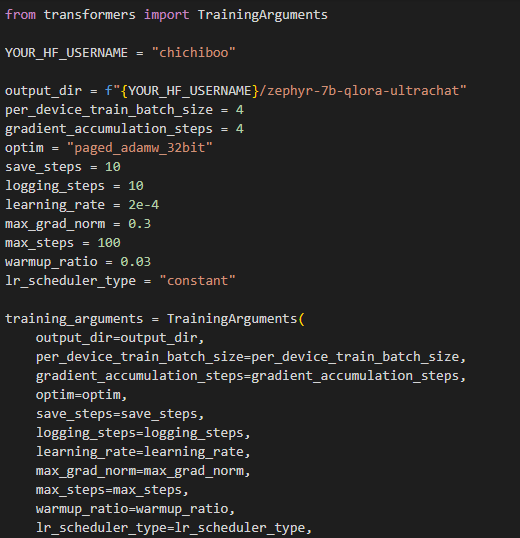
\includegraphics{qlora-snippet}
\end{figure}

This snippet is based on the fine-tuning guides available on HuggingFace and the PEFT guides on several websites.
This prototype only uses 100 iterations to train the model based on the ultrachat dataset.
Most of the parameters used in this prototype is the same with the examples but it establishes a proof of concept on the usage of Google Colab as a potential training platform and the ability of LoRA to improve generative results.

\begin{table}[h!]
	\caption{Difference between Generated Answers of the Base and LoRA Fine-Tuned Model} \vspace{0.25em}
	\centering
	\renewcommand{\arraystretch}{1.2} % Adjusts row spacing
	\begin{tabular}{@{}lp{0.85\linewidth}@{}}
		\hline
		\textbf{Before LoRA:} & \\
		USER: & Can you explain contrastive learning in machine learning in simple terms for someone new to the field of ML? \\
		ASSISTANT: & Contrastive learning is a machine learning technique that involves training a model to learn from data that is similar to the target data. The model is trained to identify patterns in the data that are similar to the target data, and to use those patterns to make predictions about new data. \\
		\hline
		\textbf{After LoRA:} & \\
		USER: & Can you explain contrastive learning in machine learning in simple terms for someone new to the field of ML? \\
		ASSISTANT: & Contrastive learning is a technique in machine learning that uses a technique called contrastive loss to train a model. The idea is to train a model to distinguish between similar and dissimilar data. In contrastive learning, a model is trained to distinguish between a pair of similar data, such as a pair of images, and a pair of dissimilar data, such as a pair of different images. The model is trained to minimize the loss, which is the difference between the similarity and dissimilarity of the data. In contrast, traditional machine learning techniques, such as supervised learning, are trained to distinguish between different types of data, such as a classification or regression task. In summary, contrastive learning is a technique in machine learning that uses a technique called contrastive loss to train a model to distinguish between similar and dissimilar data, which is different from traditional machine learning techniques, such as supervised learning. \\
		\hline
	\end{tabular}
\end{table}
